\section{Results and Discussion}
\label{sec:results}

We have \emph{combined} the different components explained in Section~\ref{sec:methodology} and we conducted a thorough experimentation process to identify the best-performing system for our task. 
By tuning the parameters of each component and selecting the optimal ones, we were able to build a 
system that addresses the persistence issue of \ac{IR} systems.
In Table~\ref{tab:map-ndcg-table}, Figure~\ref{fig:map-values} 
and Figure~\ref{fig:ndcg-values} are reported the \ac{MAP} and \ac{nDCG} scores obtained on those systems.

\newpage

\begin{table}[b]
\caption{MAP and nDCG values table}
  \label{tab:map-ndcg-table}
    \centering
    \begin{tabular}{|l|l|l|}
	\toprule
        \textbf{Run name} & \textbf{MAP value} & \textbf{nDCG value} \\
	\midrule
        FADERIC\_French-BM25-StopDefault-SnowStem & 0.211 & 0.3786 \\ 
        FADERIC\_French-LMDirichlet-Stop50-LightStem & 0.1731 & 0.3398 \\ 
        FADERIC\_French-BM25Tuned-Stop50-LightStem-Shingle-Fuzzy & 0.2383 & 0.4047 \\ 
        FADERIC\_French-BM25-Stop50-LightStem-Shingle-SpellCheck-SynCustom & 0.2404 & 0.4066 \\ 
        FADERIC\_French-BM25-Stop50-LightStem-Shingle-Fuzzy-SynCustom & 0.2416 & 0.4079 \\ 
        FADERIC\_French-BM25-Stop50-LightStem-Shingle-Fuzzy-SynCustom-Rerank20W6 & 0.2671 & 0.4274 \\ 
        FADERIC\_French-BM25-Stop50-LightStem-Shingle-Fuzzy-Rerank30  & 0.2632 & 0.423 \\ 
        FADERIC\_French-BM25-Stop50-LightStem-Shingle-Fuzzy-TrainedRerank30 & 0.1799 & 0.3599 \\ 
        FADERIC\_English-BM25-StopDefault-SnowStem & 0.149 & 0.2927 \\ 
        FADERIC\_English-LMDirichlet-Stop50-KStem & 0.1228 & 0.2612 \\ 
        FADERIC\_English-BM25-Stop50-KStem-Shingle-Fuzzy-SynPOS & 0.1634 & 0.3081 \\ 
        FADERIC\_English-BM25-Stop50-KStem-Shingle-Fuzzy-Rerank30 & 0.1873 & 0.3527 \\ 
        FADERIC\_English-BM25-Stop50-KStem-Shingle-Fuzzy-SynPOS-Rerank30 & 0.1877 & 0.3271 \\
	\bottomrule
    \end{tabular}
\end{table}

The keywords reported in the names of the runs have the following meanings:
\begin{itemize}
	\item French: used documents and queries from the French collection
	\item English: used documents and queries from the English collection
	\item BM25: used Okapi BM25 similarity (with default parameters)
	\item BM25Tuned: used Okapi BM25 similarity, with parameters tuned on training collection: k1=1.6 and b=0.7
	\item LMDirichlet: used Dirichlet smoothing (with default parameter)
	\item StopDefault: used Lucene's default stop words list
	\item Stop50: used stoplist built by picking the 50 most frequent terms in the documents indexed without stoplist and stemming
	\item LightStem: used the Light stemmer
	\item KStem: used Krovetz stemmer
	\item SnowStem: the Snowball stemmer
	\item Shingle: used word shingles (max window size = 3) query expansion
	\item Fuzzy: used fuzzyness (threshold parameter = 10) query expansion
	\item SynCustom: used custom synonyms list
	\item SynPOS: used WordNet synonym list together with OpenNLP PoS tagging
	\item SpellCheck: used the spell checker
	\item ReRerank20W6: used reranker, reranking 20 documents with weight 0.6 given to the reranker scores
	\item ReRerank30: used reranker, reranking 30 documents with weight 1 given to the reranker scores
	\item TrainedRerank30: used reranker, reranking 30 documents using our custom model
\end{itemize}

\FloatBarrier

\begin{figure}[!h]
  \centering
  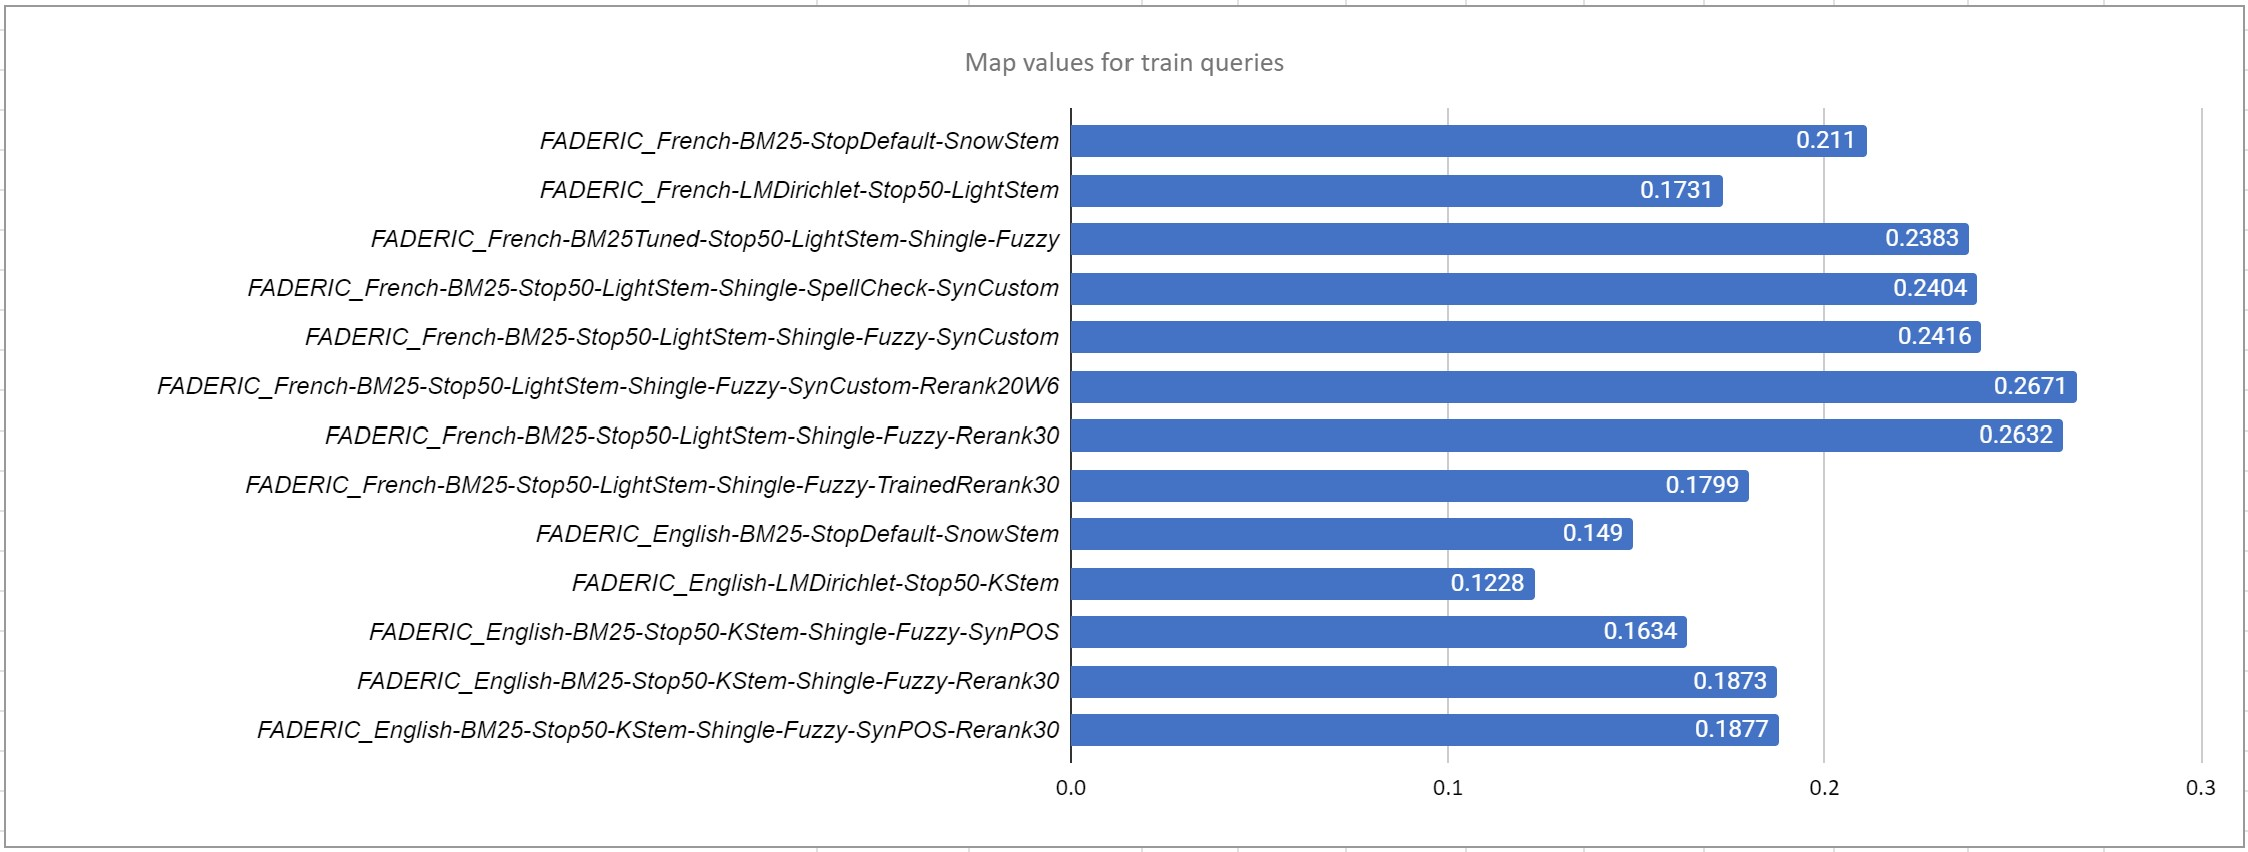
\includegraphics[width=1\linewidth]{figure/map-values.jpg}
  \caption{\ac{MAP} values table}
  \label{fig:map-values}
\end{figure}

\begin{figure}[!h]
  \centering
  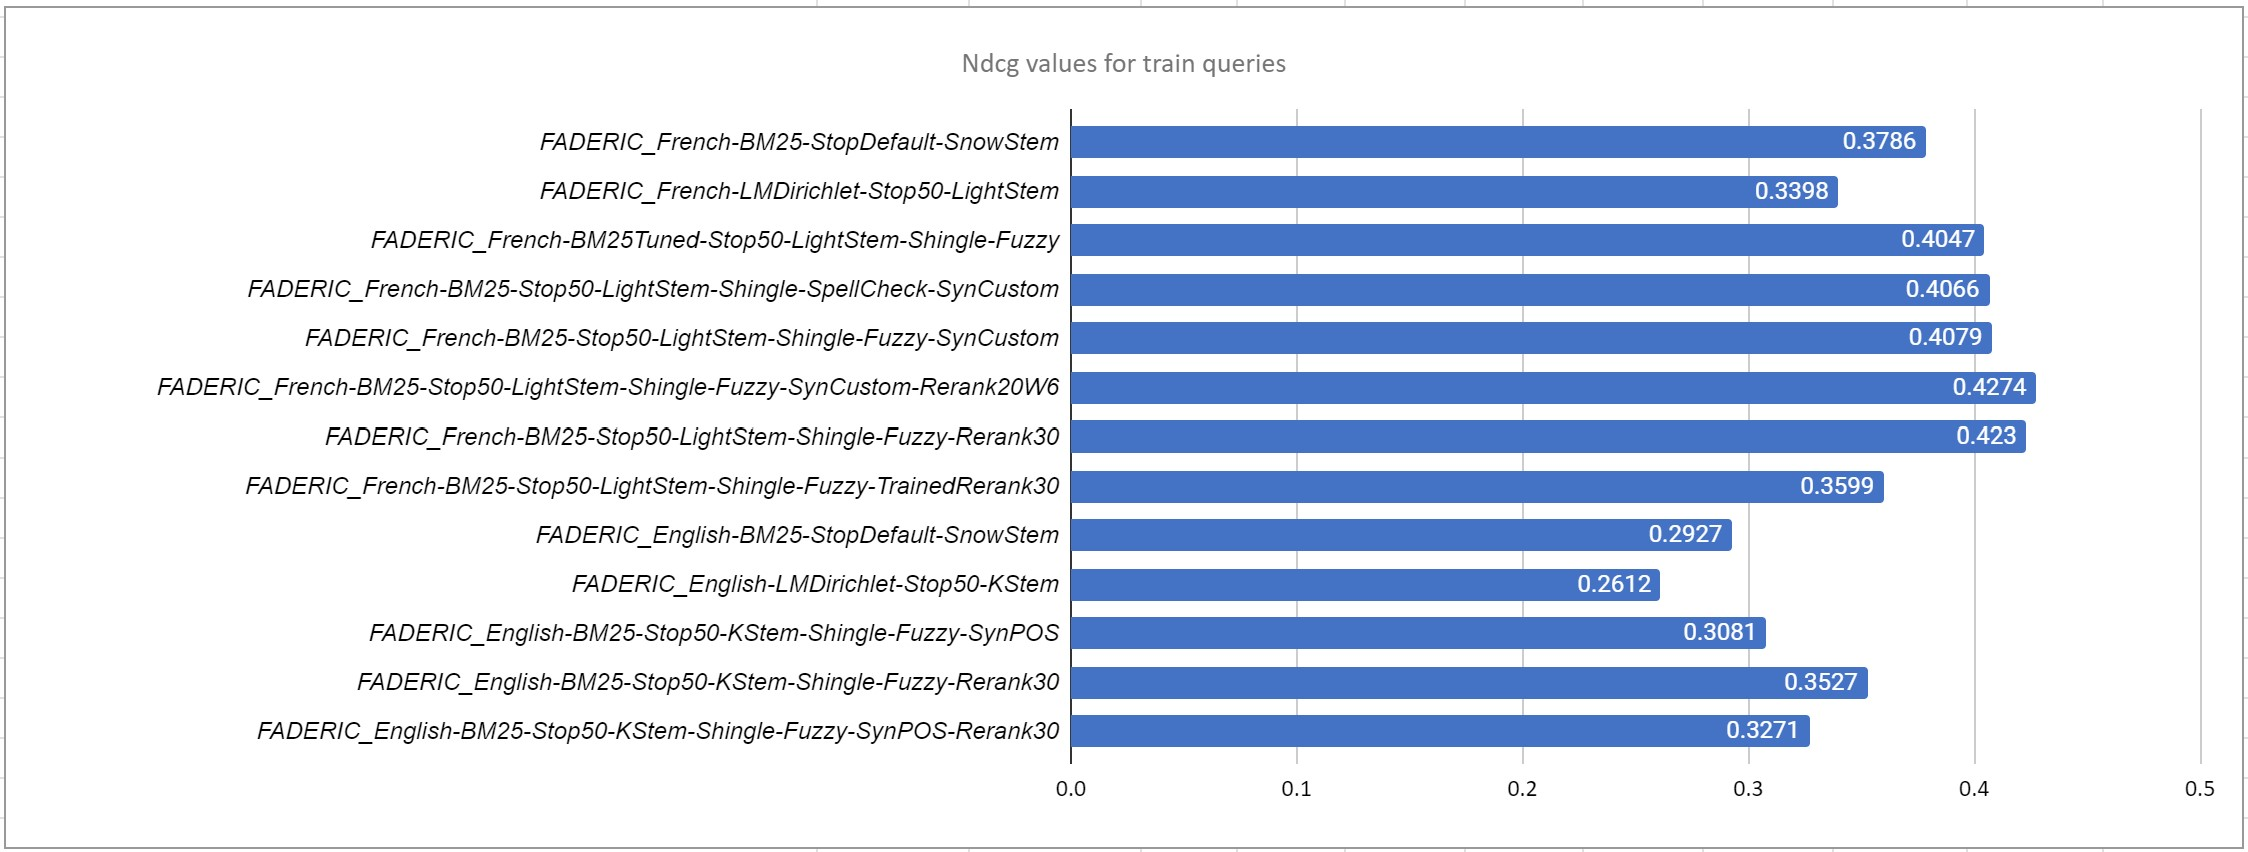
\includegraphics[width=1\linewidth]{figure/ndcg-values.jpg}
  \caption{\ac{nDCG} values table}
  \label{fig:ndcg-values}
\end{figure}

During the tuning of our system, we primarily focused on \ac{MAP} and \ac{nDCG}. However, in order to perform a more \emph{comprehensive} analysis, 
we also considered additional measures such as Precision and Recall: the first one is the fraction of retrieved 
documents that are relevant to the user's query, indicating a measure of the accuracy of the system,
while with the second is a measure of the completeness of the system in retrieving all relevant results, 
computed by the fraction of relevant documents retrieved.

In Figure~\ref{fig:precision-recall-curve}, we show the \emph{interpolated} Precision-Recall curve, which can be useful to show the inverse relationship between Precision and Recall, indicating the \emph{trade-off} between these two measures.

\begin{figure}[!h]
  \centering
  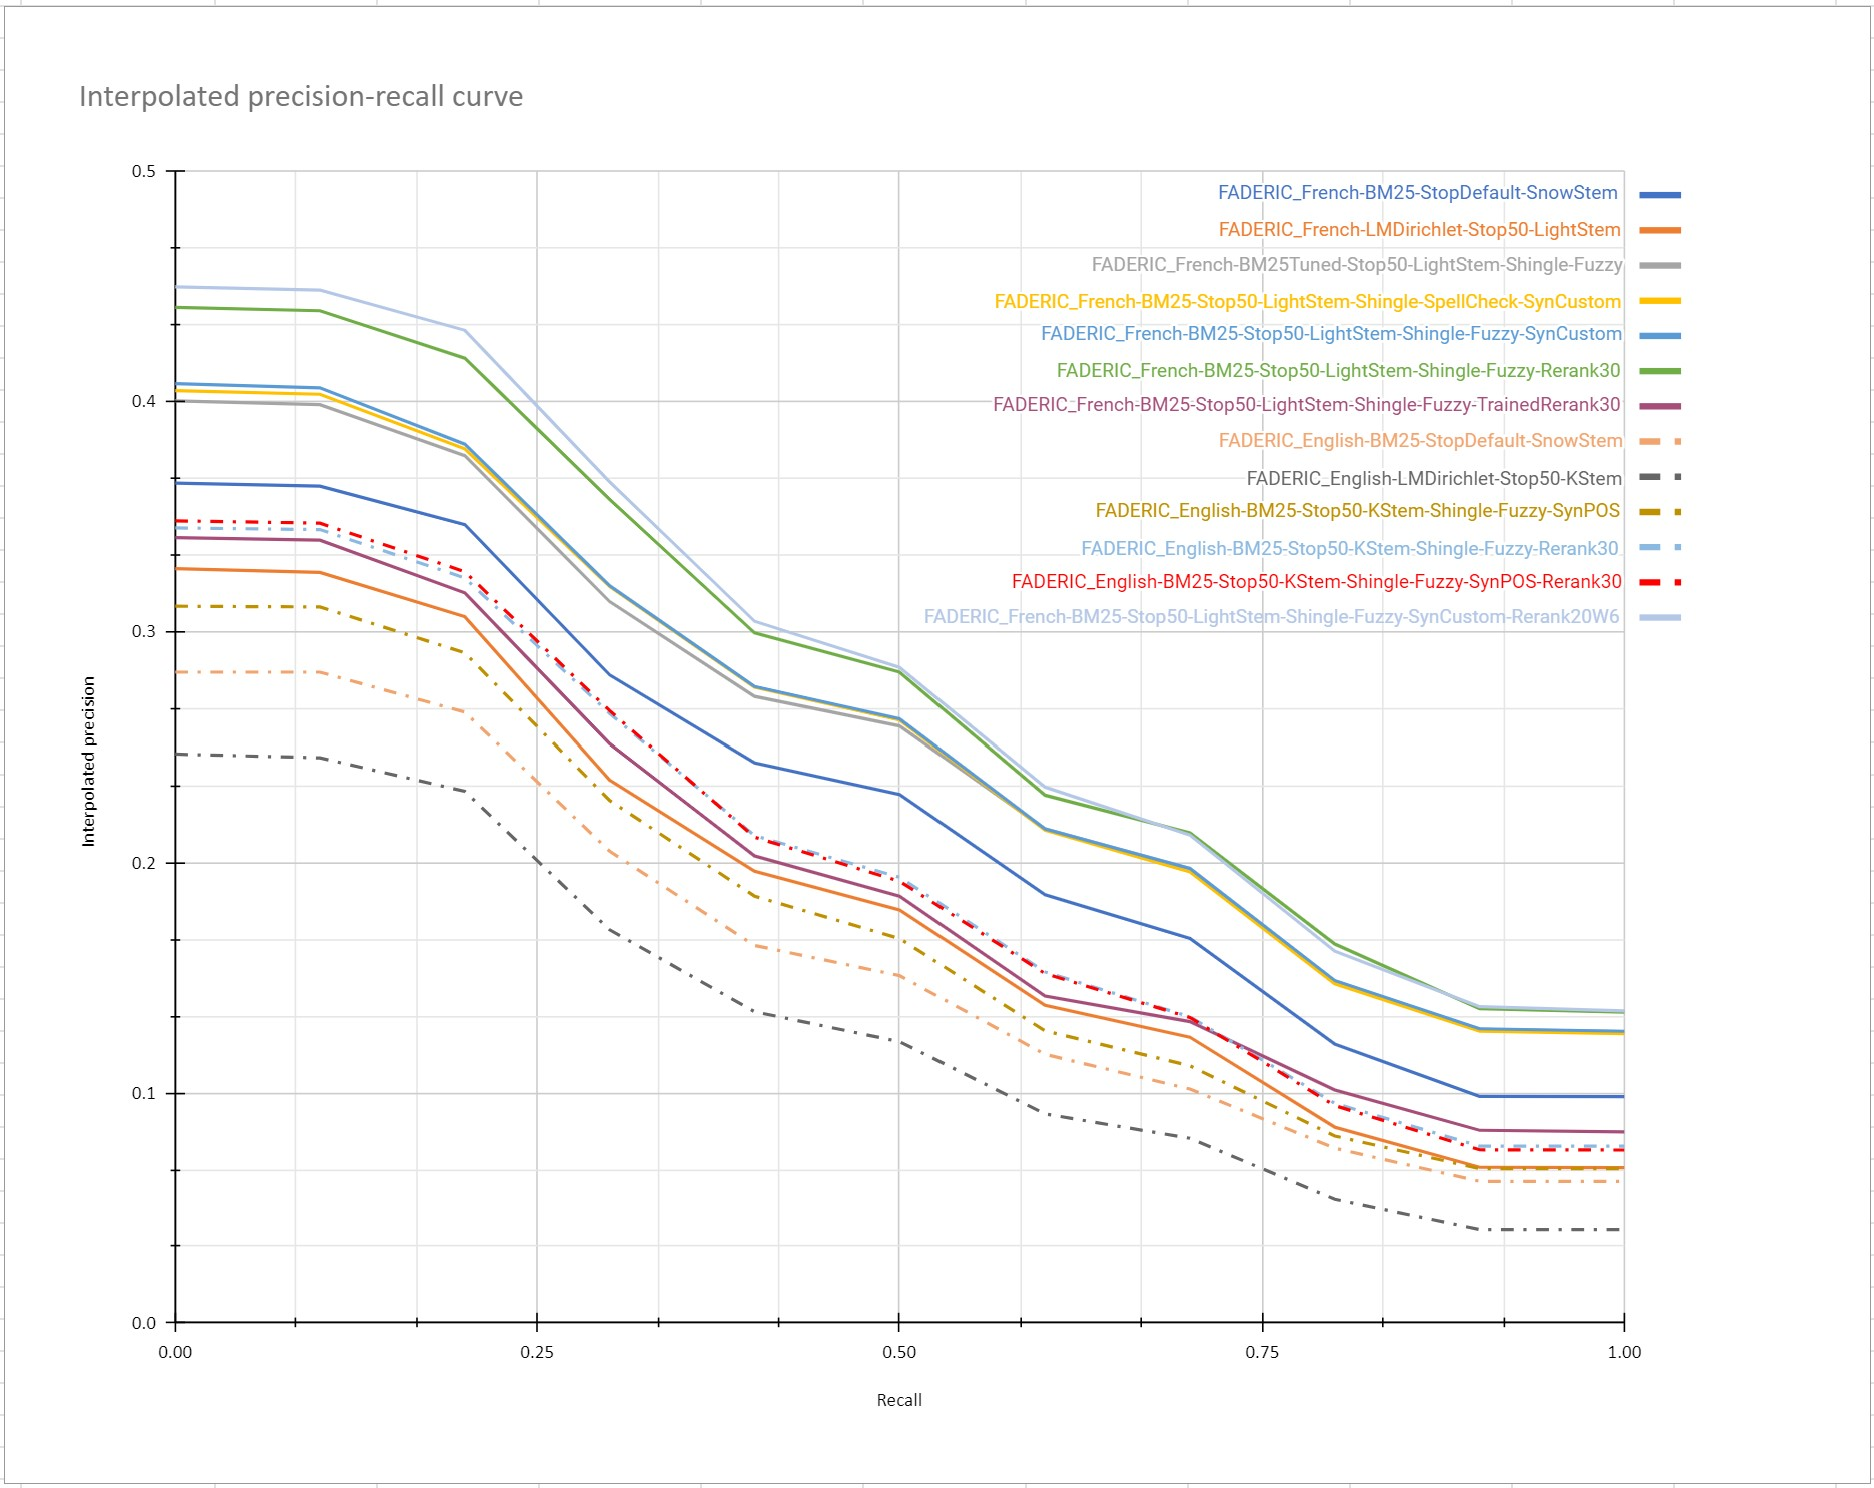
\includegraphics[width=1\linewidth]{figure/prec-recall.jpg}
  \caption{Interpolated Precision-Recall curve}
  \label{fig:precision-recall-curve}
\end{figure}

\FloatBarrier

In Table~\ref{tab:all-measures-french} and in Table~\ref{tab:all-measures-english} we have reported a more complete list of scores respectively for the French and English runs. For space reasons, we target the runs as: 

\begin{itemize}
	\item fr\_1 = FADERIC\_French-BM25-StopDefault-SnowStem
	\item fr\_2 = FADERIC\_French-LMDirichlet-Stop50-LightStem
	\item fr\_3 = FADERIC\_French-BM25Tuned-Stop50-LightStem-Shingle-Fuzzy
	\item fr\_4 = FADERIC\_French-BM25-Stop50-LightStem-Shingle-SpellCheck-SynCustom
	\item fr\_5 = FADERIC\_French-BM25-Stop50-LightStem-Shingle-Fuzzy-SynCustom
	\item fr\_6 = FADERIC\_French-BM25-Stop50-LightStem-Shingle-Fuzzy-SynCustom-Rerank20W6
	\item fr\_7 = FADERIC\_French-BM25-Stop50-LightStem-Shingle-Fuzzy-Rerank30
	\item fr\_8 = FADERIC\_French-BM25-Stop50-LightStem-Shingle-Fuzzy-TrainedRerank30
	\item en\_1 = FADERIC\_English-BM25-StopDefault-SnowStem
	\item en\_2 = FADERIC\_English-LMDirichlet-Stop50-KStem
	\item en\_3 = FADERIC\_English-BM25-Stop50-KStem-Shingle-Fuzzy-SynPOS
	\item en\_4 = FADERIC\_English-BM25-Stop50-KStem-Shingle-Fuzzy-Rerank30
	\item en\_5 = FADERIC\_English-BM25-Stop50-KStem-Shingle-Fuzzy-SynPOS-Rerank30
\end{itemize}

\begin{table}[h!]
\caption{Measures for French runs}
  \label{tab:all-measures-french}
    \centering
    \begin{tabular}{|l|l|l|l|l|l|l|l|l|l|}
    	\toprule
        runid & all & fr\_1 & fr\_2 & fr\_3 & fr\_4 & fr\_5 & fr\_6 & fr\_7 & fr\_8 \\ \midrule
        num\_q & all & 672 & 672 & 672 & 672 & 672 & 672 & 672 & 672 \\ 
        num\_ret & all & 658471 & 658512 & 660838 & 665307 & 660838 & 660838 & 660838 & 660838 \\ 
        num\_rel & all & 2626 & 2626 & 2626 & 2626 & 2626 & 2626 & 2626 & 2626 \\ 
        num\_rel\_ret & all & 2271 & 2156 & 2323 & 2311 & 2316 & 2316 & 2318 & 2318 \\ \midrule
        map & all & 0.211 & 0.1731 & 0.2383 & 0.2404 & 0.2416 & 0.267 & 0.2632 & 0.1799 \\ 
        gm\_map & all & 0.0545 & 0.0394 & 0.0696 & 0.0696 & 0.0702 & 0.0786 & 0.0765 & 0.0552 \\ \midrule
        Rprec & all & 0.1747 & 0.1469 & 0.1946 & 0.1975 & 0.1987 & 0.228 & 0.2278 & 0.1365 \\ 
        bpref & all & 0.3753 & 0.3561 & 0.4063 & 0.4079 & 0.4085 & 0.4128 & 0.4122 & 0.3701 \\ 
        recip\_rank & all & 0.3424 & 0.3134 & 0.3734 & 0.3787 & 0.3824 & 0.4222 & 0.414 & 0.317 \\ \midrule
        iprec\_at\_recall\_0.00 & all & 0.3646 & 0.3274 & 0.4003 & 0.4048 & 0.4078 & 0.4499 & 0.441 & 0.3409 \\ 
        iprec\_at\_recall\_0.10 & all & 0.3633 & 0.3258 & 0.3987 & 0.4032 & 0.406 & 0.4485 & 0.4395 & 0.3398 \\ 
        iprec\_at\_recall\_0.20 & all & 0.3465 & 0.3066 & 0.3765 & 0.3795 & 0.3815 & 0.431 & 0.4189 & 0.3169 \\ 
        iprec\_at\_recall\_0.30 & all & 0.2813 & 0.2359 & 0.3131 & 0.3197 & 0.32 & 0.3651 & 0.3575 & 0.2515 \\ 
        iprec\_at\_recall\_0.40 & all & 0.2433 & 0.1963 & 0.272 & 0.276 & 0.2763 & 0.3046 & 0.2995 & 0.203 \\ 
        iprec\_at\_recall\_0.50 & all & 0.2296 & 0.1795 & 0.2592 & 0.2618 & 0.2623 & 0.2846 & 0.2825 & 0.1855 \\ 
        iprec\_at\_recall\_0.60 & all & 0.1861 & 0.1381 & 0.2147 & 0.2141 & 0.2147 & 0.2328 & 0.2293 & 0.1421 \\ 
        iprec\_at\_recall\_0.70 & all & 0.1671 & 0.1242 & 0.1974 & 0.196 & 0.1976 & 0.212 & 0.213 & 0.131 \\ 
        iprec\_at\_recall\_0.80 & all & 0.1212 & 0.0851 & 0.1481 & 0.1474 & 0.1489 & 0.1616 & 0.1647 & 0.1013 \\ 
        iprec\_at\_recall\_0.90 & all & 0.0985 & 0.0677 & 0.1276 & 0.1269 & 0.1279 & 0.1375 & 0.1366 & 0.0838 \\ 
        iprec\_at\_recall\_1.00 & all & 0.0984 & 0.0675 & 0.1267 & 0.1258 & 0.1268 & 0.1357 & 0.1351 & 0.0831 \\ \midrule
        P\_5 & all & 0.1637 & 0.1375 & 0.1827 & 0.1866 & 0.1875 & 0.2074 & 0.2065 & 0.1315 \\ 
        P\_10 & all & 0.1332 & 0.1088 & 0.1469 & 0.1463 & 0.1472 & 0.1603 & 0.156 & 0.1007 \\ 
        P\_15 & all & 0.109 & 0.0889 & 0.1167 & 0.1176 & 0.1183 & 0.1233 & 0.1243 & 0.0869 \\ 
        P\_20 & all & 0.0901 & 0.0753 & 0.099 & 0.0986 & 0.099 & 0.099 & 0.1022 & 0.0799 \\ 
        P\_30 & all & 0.0683 & 0.058 & 0.0743 & 0.0746 & 0.0748 & 0.0748 & 0.0743 & 0.0742 \\ 
        P\_100 & all & 0.0267 & 0.0232 & 0.028 & 0.0279 & 0.0279 & 0.0279 & 0.0279 & 0.0279 \\ 
        P\_200 & all & 0.0146 & 0.0133 & 0.0151 & 0.015 & 0.015 & 0.015 & 0.015 & 0.015 \\ 
        P\_500 & all & 0.0064 & 0.006 & 0.0065 & 0.0065 & 0.0065 & 0.0065 & 0.0065 & 0.0065 \\ 
        P\_1000 & all & 0.0034 & 0.0032 & 0.0035 & 0.0034 & 0.0034 & 0.0034 & 0.0034 & 0.0034 \\ \midrule
        recall\_5 & all & 0.2106 & 0.1802 & 0.2417 & 0.2477 & 0.2478 & 0.2738 & 0.2732 & 0.1749 \\ 
        recall\_10 & all & 0.3402 & 0.2789 & 0.3828 & 0.3813 & 0.383 & 0.4167 & 0.4042 & 0.2606 \\ 
        recall\_15 & all & 0.4203 & 0.338 & 0.4499 & 0.454 & 0.456 & 0.4724 & 0.4757 & 0.3366 \\ 
        recall\_20 & all & 0.4595 & 0.3814 & 0.5051 & 0.5016 & 0.5032 & 0.5034 & 0.5193 & 0.4119 \\ 
        recall\_30 & all & 0.5187 & 0.4412 & 0.5677 & 0.5703 & 0.571 & 0.571 & 0.5657 & 0.5651 \\ 
        recall\_100 & all & 0.6688 & 0.5816 & 0.7028 & 0.7019 & 0.7022 & 0.7022 & 0.7019 & 0.7019 \\ 
        recall\_200 & all & 0.7283 & 0.6729 & 0.7587 & 0.7553 & 0.7555 & 0.7555 & 0.756 & 0.756 \\ 
        recall\_500 & all & 0.7994 & 0.7574 & 0.8235 & 0.8217 & 0.8219 & 0.8219 & 0.8232 & 0.8232 \\ 
        recall\_1000 & all & 0.8485 & 0.8072 & 0.8685 & 0.8656 & 0.8663 & 0.8663 & 0.8662 & 0.8662 \\ \midrule
        ndcg & all & 0.3786 & 0.3398 & 0.4047 & 0.4066 & 0.4079 & 0.4274 & 0.423 & 0.3599 \\
	\bottomrule
    \end{tabular}
\end{table}

\FloatBarrier


\begin{table}[p]
\caption{Measures for English runs}
  \label{tab:all-measures-english}
    \centering
    \begin{tabular}{|l|l|l|l|l|l|l|}
    \toprule
        runid & all & en\_1 & en\_2 & en\_3 & en\_4 & en\_5 \\ \midrule
        num\_q & all & 671 & 671 & 672 & 672 & 672 \\ 
        num\_ret & all & 654919 & 654764 & 655602 & 655602 & 655602 \\ 
        num\_rel & all & 2623 & 2623 & 2626 & 2626 & 2626 \\ 
        num\_rel\_ret & all & 1878 & 1765 & 1924 & 1915 & 1924 \\ \midrule
        map & all & 0.149 & 0.1228 & 0.1634 & 0.1873 & 0.1877 \\ 
        gm\_map & all & 0.0164 & 0.0122 & 0.0195 & 0.0215 & 0.0221 \\ \midrule
        Rprec & all & 0.1253 & 0.1092 & 0.1385 & 0.1708 & 0.1706 \\ 
        bpref & all & 0.3263 & 0.3139 & 0.3417 & 0.3524 & 0.3536 \\ 
        recip\_rank & all & 0.2697 & 0.2364 & 0.2967 & 0.3289 & 0.3322 \\ \midrule
        iprec\_at\_recall\_0.00 & all & 0.2825 & 0.2471 & 0.3111 & 0.3451 & 0.3482 \\ 
        iprec\_at\_recall\_0.10 & all & 0.2825 & 0.2455 & 0.3108 & 0.3444 & 0.3472 \\ 
        iprec\_at\_recall\_0.20 & all & 0.2652 & 0.231 & 0.2909 & 0.3234 & 0.3261 \\ 
        iprec\_at\_recall\_0.30 & all & 0.205 & 0.1709 & 0.227 & 0.2646 & 0.2658 \\ 
        iprec\_at\_recall\_0.40 & all & 0.1641 & 0.1353 & 0.1855 & 0.2118 & 0.2111 \\ 
        iprec\_at\_recall\_0.50 & all & 0.151 & 0.1223 & 0.1671 & 0.1937 & 0.192 \\ 
        iprec\_at\_recall\_0.60 & all & 0.1168 & 0.0909 & 0.127 & 0.1526 & 0.1519 \\ 
        iprec\_at\_recall\_0.70 & all & 0.1017 & 0.0803 & 0.1118 & 0.1331 & 0.1328 \\ 
        iprec\_at\_recall\_0.80 & all & 0.076 & 0.0538 & 0.0813 & 0.0955 & 0.0945 \\ 
        iprec\_at\_recall\_0.90 & all & 0.0616 & 0.0406 & 0.0671 & 0.0769 & 0.0753 \\ 
        iprec\_at\_recall\_1.00 & all & 0.0616 & 0.0406 & 0.0671 & 0.0769 & 0.0752 \\ \midrule
        P\_5 & all & 0.1195 & 0.1019 & 0.1345 & 0.1542 & 0.1542 \\ 
        P\_10 & all & 0.0954 & 0.0793 & 0.1042 & 0.1131 & 0.1137 \\ 
        P\_15 & all & 0.0784 & 0.065 & 0.0835 & 0.0898 & 0.0904 \\ 
        P\_20 & all & 0.0662 & 0.0543 & 0.0705 & 0.0732 & 0.0745 \\ 
        P\_30 & all & 0.0513 & 0.0433 & 0.0537 & 0.053 & 0.0536 \\ 
        P\_100 & all & 0.0201 & 0.0179 & 0.0208 & 0.0209 & 0.0208 \\ 
        P\_200 & all & 0.0113 & 0.0103 & 0.0116 & 0.0115 & 0.0116 \\ 
        P\_500 & all & 0.0051 & 0.0048 & 0.0052 & 0.0052 & 0.0052 \\ 
        P\_1000 & all & 0.0028 & 0.0026 & 0.0029 & 0.0028 & 0.0029 \\ 
        recall\_5 & all & 0.1512 & 0.1329 & 0.171 & 0.2017 & 0.202 \\ 
        recall\_10 & all & 0.2437 & 0.1988 & 0.2628 & 0.2887 & 0.2909 \\ 
        recall\_15 & all & 0.297 & 0.2432 & 0.3155 & 0.3404 & 0.343 \\ 
        recall\_20 & all & 0.3318 & 0.2727 & 0.3523 & 0.3683 & 0.3745 \\ 
        recall\_30 & all & 0.3861 & 0.3281 & 0.4018 & 0.397 & 0.401 \\ 
        recall\_100 & all & 0.5 & 0.4486 & 0.5151 & 0.5167 & 0.514 \\ 
        recall\_200 & all & 0.563 & 0.518 & 0.5774 & 0.5754 & 0.5769 \\ 
        recall\_500 & all & 0.6443 & 0.6087 & 0.6612 & 0.6597 & 0.6607 \\ 
        recall\_1000 & all & 0.7027 & 0.6635 & 0.7186 & 0.715 & 0.7186 \\ \midrule
        ndcg & all & 0.2927 & 0.2612 & 0.3081 & 0.3257 & 0.3271 \\ \bottomrule
    \end{tabular}
\end{table}

\FloatBarrier

Based on these results, we can derive the following considerations:

\begin{itemize}
	\item the runs on the French collections are significantly better than the ones on the English one, the reason for this is the \emph{automatic translation} of the document collection, which has led to errors and inconsistencies in the English one;
which has resulted in errors and inconsistencies in the English collection. 
	\item the system performs better when configured to use BM25 similarity instead of the Dirichlet smoothing;
	\item the \emph{tuned} parameters on BM25 just gave slightly betters results, probably \emph{overfitting} the run we have tuned them on, for this reason we have chosen to use the default ones in most of the runs;
	\item the custom stoplist we have generated by picking the most frequent terms has outperformed Lucene's default ones because since it was based on the specific collection the \emph{effectivness} of using a stoplist has been maximized;
	\item in both French and English the Snowball stemmer performed worse than the Light and Krovetz stemmer, respectevly;
	\item fuzzyness and spell checking have given similar results but the first one was slightly better, probably because the spell checker is dictionary based and thus \emph{not flexible} for non conventional words;
	\item the use of shingles improved the performances, allowing to have more \emph{contextual matches} by looking for group of words instead of single ones;
	\item synonyms have slightly improved the performances, this is due to the fact that sometimes they can be \emph{misleading} and retrieve documents that are not contextual with the query;
	\item the reranking is a very \emph{powerful} tool that has given a huge performance increase to our runs.
\end{itemize}

Based on the previous results and these considerations, we have decided to submit to \ac{CLEF} the following systems:
\begin{itemize}
	\item FADERIC\_French-BM25-Stop50-LightStem-Shingle-Fuzzy-SynCustom-Rerank20W6, i.e., the best system overall;
	\item FADERIC\_English-BM25-Stop50-KStem-Shingle-Fuzzy-SynPOS-Rerank30, i.e., the best system overall on the English collection;
	\item FADERIC\_French-BM25-Stop50-LightStem-Shingle-Fuzzy-SynCustom, i.e., the best system without the use of reranking;
	\item FADERIC\_French-BM25-Stop50-LightStem-Shingle-Fuzzy-Rerank30, i.e., the best system without the use of synonyms;
	\item FADERIC\_French-BM25Tuned-Stop50-LightStem-Shingle-Fuzzy, i.e., the best system without the use of both synonyms and reranking;

\end{itemize}
